%
%
%
\section{Cadmium Telluride Sensor}
\label{sec:siliconpad}
%Fig: Quantum Efficiency vs wavelength
%Photos of sensor, drawing for the circuit

Cadmium-telluride features a significantly large efficiency for photons in the energy range between 10 keV and 100 keV and beyond compared to silicon sensors. The higher atomic number of Cadmium and Tellurium results in a higher cross section for photons in this energy range. 
Photons in this energy range are abundant in electromagnetic showers \cite{showercomposition}. 
Furthermore are Cadmium-Tellurium sensors available with a thickness of the active layer of 1 mm and more.  
%
Our measurements were conducted with a CdTe Schottky type diode purchased from Acrorad \cite{acrorad}. It is $1 cm^2$ in size transversely and 1 mm thick.
It was operated at a bias voltage of 700 V, the dark current was between 3 nA and 6 nA depending on the environmental conditions in the test beam experimental zones.     
%
\begin{figure}[htbp] 
\centering
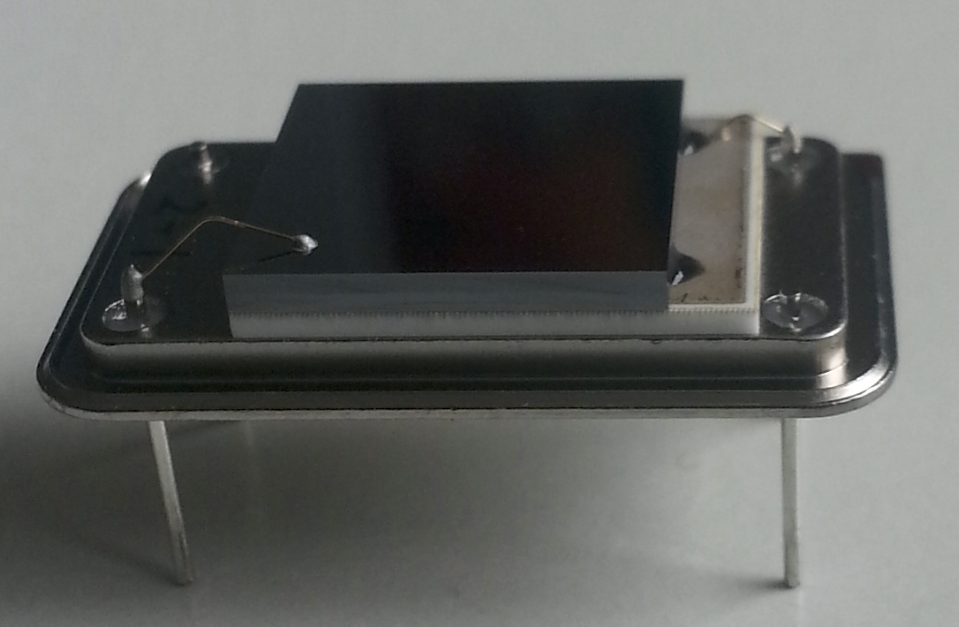
\includegraphics[width=0.49\textwidth]{figures/CdTeSensor.png} 
\caption{Cadmium-Tellurid sensor used in the setup. The sensor is a Shotky type diode with a transverse size of $1 cm^2$ and a thicknees of 1 mm. It is biased at 700 V.} 
\label{fig:CdTeSensor} 
\end{figure} 
%
The sensor was placed in a box made of 0.3 mm copper sheets sealed with copper tape. 
The electrical circuit shown in Fig.~\ref{fig:cdtecircuit} was used to connect to the sensor to the bias voltage with a standard high voltage cable and the readout electronics using a SMA cable with a feed through penetrating the copper box.
A high bandwidth amplifier from Hamamatsu with an amplification of 36 dB was used amplify the output signal of the CdTe sensor.
An attenuator of 10 dB was used to attenuate the input signal to the amplifier to adjust the CdTe signal to the dynamic range of the amplifier.
The output of the amplifier was fed into a CAEN V1742 digitizer operated at 5 GS/s.
%
\begin{figure}[htbp] 
\centering
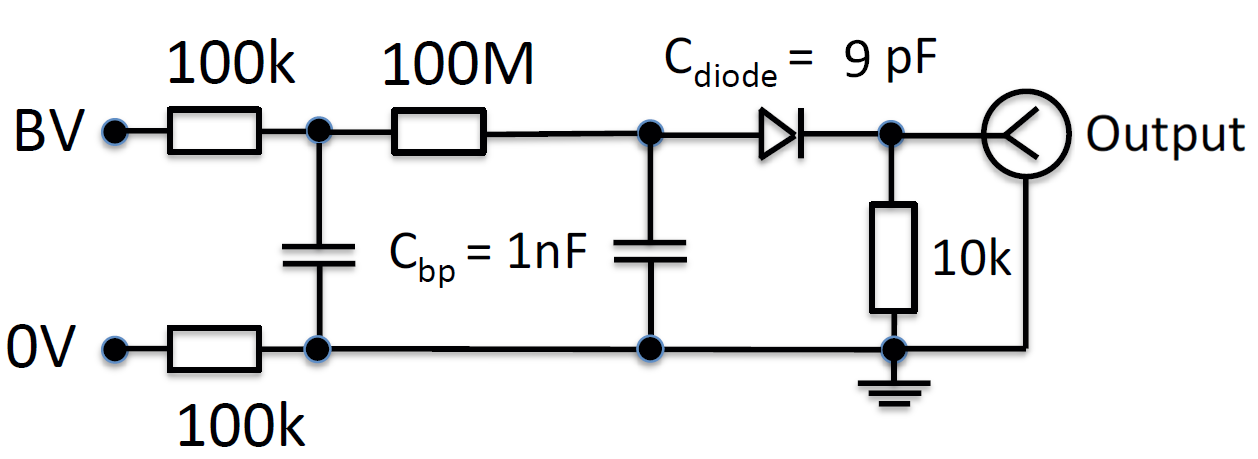
\includegraphics[width=0.49\textwidth]{figures/circuit_CdTe.png} 
\caption{Circuit to connect the Cadmium-Telluride sensor to the high voltage (BV) and the signal output. The circuit is mounted inside a copper box with the sensor.} 
\label{fig:cdtecircuit} 
\end{figure} 
%
